% Literatura Cinza - protocolo, resultados, lista de ferramentas encontradas -> lista preliminar de requisitos
% Screenshot / análise / resumo sobre 
%==============================================================================
\chapter{Gray Literature}\label{grayliterature}
%==============================================================================

Since the final outcome of this research is a software product, a systematic review of the gray literature - to map and evaluate existing tools and solutions that already solve the problem of managing outreach activities in the context of higher education universities - would be of great value before starting the development of the solution itself. The review was conducted by two authors. As previously mentioned, there are two research papers, written individually, but the artifacts created to support the study were made in conjunction.

This chapter reports the systematic review carried out in the gray literature. In addition, information relevant to the development of the goal product, obtained through the research, will also be presented. The protocol defined to conduct the review will be discussed, citing points such as research questions, inclusion and exclusion criteria, extracted data and search strings, in addition to detailed analysis and comparisons of the selected tools.

The article is organized as follows: The \autoref{sec:gl-background} introduces terms and concepts used during the study. In \autoref{sec:gl-planning}, the protocol defined by the authors will be presented. How the research was conducted, together with the data collected to answer the research questions will be described in \autoref{sec:gl-reporting} and \autoref{sec:gl-validity} discusses threats to the validity of the study. Finally, \autoref{sec:gl-considerations} completes the systematic review.

\section{Background}\label{sec:gl-background}

Gray literature is defined by the following quote from \cite{garousi2019guidelines}: "<gray literature> is produced at all levels of government, academia, business, and industry in print and electronic formats, but is not controlled by commercial publishers, or that is, where publication is not the main activity of the producing body".

The term ``black box'' refers to the quality of software where the internal mechanisms of the system are not known; its use only focuses on outputs generated in response to selected inputs and execution conditions \cite{nidhra2012black}. This term was used in the context of the Google search engine, where it is not known exactly what happens internally, only that sometimes the results vary minimally, even though the search string remains the same.

\section{Planning}\label{sec:gl-planning}

The authors decided that it would be more interesting and add more value to the study if a systematic review was carried out in the gray literature instead of in the white literature, due to the little content of formal works published on the outreach activities management topic.

\subsection{Reasons for carrying out the review}\label{sec:gl-planning-motives}

The main reasons to include a gray literature in review in the study by the authors were the following:
\begin{inparaenum}[(i)]
  \item More search results for tools instead of formal articles;
  \item Running the search strings on white literature returned very few results;
  \item Several tools and solutions do not have published articles;
  \item By searching for tools, the authors hope to find functionality ideas and inspiration for the development of the goal product itself.
\end{inparaenum}

In the \autoref{tab:questoesgarousi} are the questions used in the decision to carry out the review of the gray literature and their answers. In addition, the objectives defined for carrying out the review were:

\begin{inparaenum}[(i)]
  \item Find free tools that partially support academic management;
  \item Find features in existing tools;
  \item Validate ideas for features and data that will be used in the solution.
\end{inparaenum}

\begin{table}
  \centering
  \caption{Questions for inclusion of gray literature}
  \label{tab:questoesgarousi}
  \resizebox{\textwidth}{!}{
    \begin{tabular}{|l|c|}
      \hline
      \rowcolor[rgb]{0.753,0.753,0.753} \multicolumn{1}{|c|}{Question}                                                                                                          & Answer \\
      \hline
      Is the subject “complex” and insoluble considering only the formal literature?                                                                                            & No     \\
      \hline
      \begin{tabular}[c]{@{}l@{}}Is there a lack of volume or quality of evidence, or lack of consensus on outcome measurement in the \\formal literature?\end{tabular}         & Yes    \\
      \hline
      Is contextual information important to the subject under study?                                                                                                           & Yes    \\
      \hline
      Is the objective to validate or corroborate scientific results with practical experiences?                                                                                & No     \\
      \hline
      Is the aim to challenge assumptions or falsify results of practice using academic research or vice versa?                                                                 & No     \\
      \hline
      \begin{tabular}[c]{@{}l@{}}Would a synthesis of insights and evidence from the industrial and academiccommunity be useful to one \\or even both communities?\end{tabular} & Yes    \\
      \hline
      Is there a large volume of professional sources that indicate high professional interest in a topic?                                                                      & Yes    \\
      \hline
    \end{tabular}
  }
  \fonte{Adapted from \cite{garousi2019guidelines}.}
\end{table}

\subsection{Research questions}\label{sec:gl-planning-rq}

In \autoref{tab:research-questions} are presented the research questions defined by the authors to be answered with the systematic review.

\begin{table}
  \centering
  \caption{Research Questions}
  \label{tab:research-questions}
  \resizebox{\textwidth}{!}{
    \begin{tabular}{|l|l|}
      \hline
      \rowcolor[rgb]{0.753,0.753,0.753} \multicolumn{1}{|c|}{ID} & \multicolumn{1}{c|}{Question}                                                                         \\
      \hline
      RQ 1.                                                      & What tools currently exist that perform academic management?                                          \\
      \hline
      RQ 1.1.                                                    & Which ones have related functionality or support outreach activities?                                 \\
      \hline
      RQ 1.2.                                                    & What are the features offered by these tools?                                                         \\
      \hline
      RQ 1.3.                                                    & What are the most common features between this type of tool?                                          \\
      \hline
      RQ 1.4.                                                    & What data do the tools use in relation to activities, participant registration and user registration? \\
      \hline
    \end{tabular}
  }
  \fonte{Author.}
\end{table}

\subsection{Search strings}\label{sec:gl-planning-strings}

The search strings were created after adapting the methodology used in \cite{godin2015applying}. First, search terms were created, using keywords such as \textbf{extensão} (outreach), \textbf{programa} (program), \textbf{projeto} (project), \textbf{gerenciamento} (management) and \textbf{atividade} (activity).

Furthermore, due to the scope being limited to outreach activities in Brazilian universities, the site filter provided by the search engine used ``site:.edu.br'' was initially used, meaning that only sites whose domain included the specified ending would be shown. However, it was later realized that it was better to remove the filter as some private universities do not have .edu in their domain.

Ultimately, the authors came up with ten search strings in total, with seven of them using the combination of the terms "\textbf{extensão} (\textbf{programa} | \textbf{projeto})", which were defined as the most relevant terms. With each string, a limit was set to use only the first ten pages returned by the search engine, resulting in one hundred records per string and, consequently, one thousand records in total.

The keyword ``\acs{SIGAA}'' was removed after the first search because it is a tool used by many public universities, which cluttered the results with essentially the same record, potentially hiding other solutions. The defined strings are presented in \autoref{tab:gl-strings}.

\begin{table}
  \centering
  \caption{Search Strings}
  \label{tab:gl-strings}
  \resizebox{\textwidth}{!}{
    \begin{tabular}{|c|l|}
      \hline
      \rowcolor[rgb]{0.753,0.753,0.753} No. & \multicolumn{1}{c|}{Search String}                                                                                          \\
      \hline
      1                                     & sistema gestão acadêmicas (atividades \textbar{} projetos) site:.edu.br                                                     \\
      \hline
      2                                     & (sistema \textbar{} ferramenta) gestão acadêmicas (atividades \textbar{} projetos) extensão site:.edu.br -SIGAA             \\
      \hline
      3                                     & (ferramenta \textbar{} aplicação) extensão (programa \textbar{} projeto) (gestão \textbar{} gerenciamento) -SIGAA           \\
      \hline
      4                                     & (app \textbar{} aplicativo) extensão (programa \textbar{} projeto) (administração \textbar{} gerência) -SIGAA               \\
      \hline
      5                                     & ferramenta extensão (programa \textbar{} projeto) (gestão \textbar{} gerência) -SIGAA                                       \\
      \hline
      6                                     & (ferramenta \textbar{} aplicação \textbar{} app \textbar{} aplicativo) extensão (programa \textbar{} projeto) gestão -SIGAA \\
      \hline
      7                                     & software extensão (programa \textbar{} projeto) (gerência \textbar{} gestão \textbar{} controle) -SIGAA                     \\
      \hline
      8                                     & (software \textbar{} ferramenta \textbar{} aplicação) extensão atividade -SIGAA                                             \\
      \hline
      9                                     & sistema extensão (projeto \textbar{} programa \textbar{} atividade) gestão -SIGAA                                           \\
      \hline
      10                                    & acadêmica extensão (projeto \textbar{} programa \textbar{} atividade) -SIGAA                                                \\
      \hline
    \end{tabular}
  }
  \fonte{Author.}
\end{table}

The search for the strings itself was performed on the Google search engine.

\subsection{Inclusion criteria}\label{sec:gl-planning-inc}

The elaboration of the inclusion criteria took place in two stages. Due to the large number of institutional sites that were just catalogs of outreach activities, in the first stage the authors applied a filter to differentiate tools from catalogs. To be included, the result should include at least three of the following criteria:
\begin{inparaenum}[(a)]
  \item User login;
  \item Registration of activities;
  \item Activity listing;
  \item Possibility of signing up for outreach activities.
\end{inparaenum}

After filtering the results with the criteria established above, step 2 was applied. In it, the criteria defined for inclusion were more rigorous. They are presented in \autoref{tbl:gl-inclusion-criteria}:

\begin{table}
  \centering
  \caption{Inclusion Criteria}
  \label{tbl:gl-inclusion-criteria}
  \resizebox{\textwidth}{!}{
    \begin{tabular}{|c|l|}
      \hline
      \rowcolor[rgb]{0.753,0.753,0.753} ID & \multicolumn{1}{c|}{Inclusion Criteria}                              \\
      \hline
      IC 1.                                & The tool or website supports the management of extension activities. \\
      \hline
      IC 2.                                & The tool or website has a stable version.                            \\
      \hline
      IC 3.                                & If it is a tool, it must have documentation.                         \\
      \hline
    \end{tabular}
  }
  \fonte{Author.}
\end{table}

\subsection{Exclusion criteria}\label{sec:gl-planning-exc}

In addition to applying the inclusion criteria, exclusion criteria were also defined, in which any result that fit only one of them was automatically excluded from the review. Initially, the authors defined a total of 6 criteria, however, after alignments with the advisor, it was realized that two of them were unnecessary. The rest, which were applied to the results, are displayed in \autoref{tbl:gl-exclusion-criteria}.

\begin{table}
  \centering
  \caption{Exclusion Criteria}
  \label{tbl:gl-exclusion-criteria}
  \resizebox{\textwidth}{!}{
    \begin{tabular}{|c|l|}
      \hline
      \rowcolor[rgb]{0.753,0.753,0.753} ID & \multicolumn{1}{c|}{Exclusion Criteria}                                                                   \\
      \hline
      EC 1.                                & If it is a tool, it does not have a source code download or an online page.                               \\
      \hline
      EC 2.                                & The tool or the website has not received updates for more than 10 years.                                  \\
      \hline
      EC 3.                                & The tool or website is for the exclusive use of the organization, that is, closed to the external public. \\
      \hline
      EC 4.                                & The tool or website is paid and does not provide a trial version or all outreach activities are paid.     \\
      \hline
    \end{tabular}
  }
  \fonte{Author.}
\end{table}

\subsection{Quality criteria}\label{sec:gl-planning-qlty}

To assess the quality of the tools that passed the inclusion and exclusion criteria, five quality criteria were defined that are focused on characteristics considered important within a tool and how it stands out from the others. To quantify the scores for each criterion, the scale used in the article by \cite{iung2020systematic} was adapted, being:
\begin{inparaenum}[(i)]
  \item \textbf{Y}es: 1.0;
  \item \textbf{P}artially: 0.5;
  \item \textbf{N}o: 0.
\end{inparaenum}
The defined criteria are presented in \autoref{tbl:gl-quality-criteria}.

\begin{table}
  \centering
  \caption{Quality Criteria}
  \label{tbl:gl-quality-criteria}
  \arrayrulecolor{black}
  \resizebox{\textwidth}{!}{
    \begin{tabular}{|c|l|r|c|l|}
      \hline
      \rowcolor[rgb]{0.753,0.753,0.753} {\cellcolor[rgb]{0.753,0.753,0.753}}                     & \multicolumn{1}{c|}{{\cellcolor[rgb]{0.753,0.753,0.753}}}                                                             & \multicolumn{3}{c|}{Score}                                                                            \\
      \hhline{|>{\arrayrulecolor[rgb]{0.753,0.753,0.753}}-->{\arrayrulecolor{black}}---|}
      \rowcolor[rgb]{0.753,0.753,0.753} \multirow{-2}{*}{{\cellcolor[rgb]{0.753,0.753,0.753}}ID} & \multicolumn{1}{c|}{\multirow{-2}{*}{{\cellcolor[rgb]{0.753,0.753,0.753}}Quality Criteria}}                           & \multicolumn{1}{c|}{Yes (1)} & Partially (0.5)                & \multicolumn{1}{c|}{No (0)}           \\
      \hline
      QC 1.                                                                                      & \begin{tabular}[c]{@{}l@{}}Does the tool use a relevant amount of data \\related to outreach activities?\end{tabular} & The tool uses... >=20        & 10 - 19                        & 10 pieces of information              \\
      \hline
      QC 2.                                                                                      & \begin{tabular}[c]{@{}l@{}}Does the tool have unique features among \\the selected tools?\end{tabular}                & The tool has 1               & 1                              & 0 unique features                     \\
      \hline
      QC 3.                                                                                      & \begin{tabular}[c]{@{}l@{}}Does the tool have a relevant amount of \\features among those collected?\end{tabular}     & The tool has >=14            & 9-13                           & 8 features in common with other tools \\
      \hline
      \multicolumn{1}{|l|}{QC 4.}                                                                & Does the tool have specialized support?                                                                               & Yes                          & Only FAQ                       & No                                    \\
      \hline
      \multicolumn{1}{|l|}{QC 5.}                                                                & Has the tool been maintained frequently?                                                                              & The last update was in 2022  & \multicolumn{1}{l|}{2021-2019} & before 2019                           \\
      \hline
    \end{tabular}
  }
  \fonte{Author.}
\end{table}

\subsection{Data extraction strategy}\label{sec:gl-planning-datastrategy}

In order to answer the defined research questions (\autoref{tab:research-questions}), after the final list of tools is selected, a manual data extraction is carried out. Initially, we seek all the functionalities related to \ac{OA} that the tool provides, generating a matrix with the data. There, all the different functionalities found between the results are listed. The matrix can be seen in \autoref{fig:gl-matrix}.

\begin{figure}[htb]
  \caption{Feature Matrix}\label{fig:gl-matrix}
  \begin{center}
    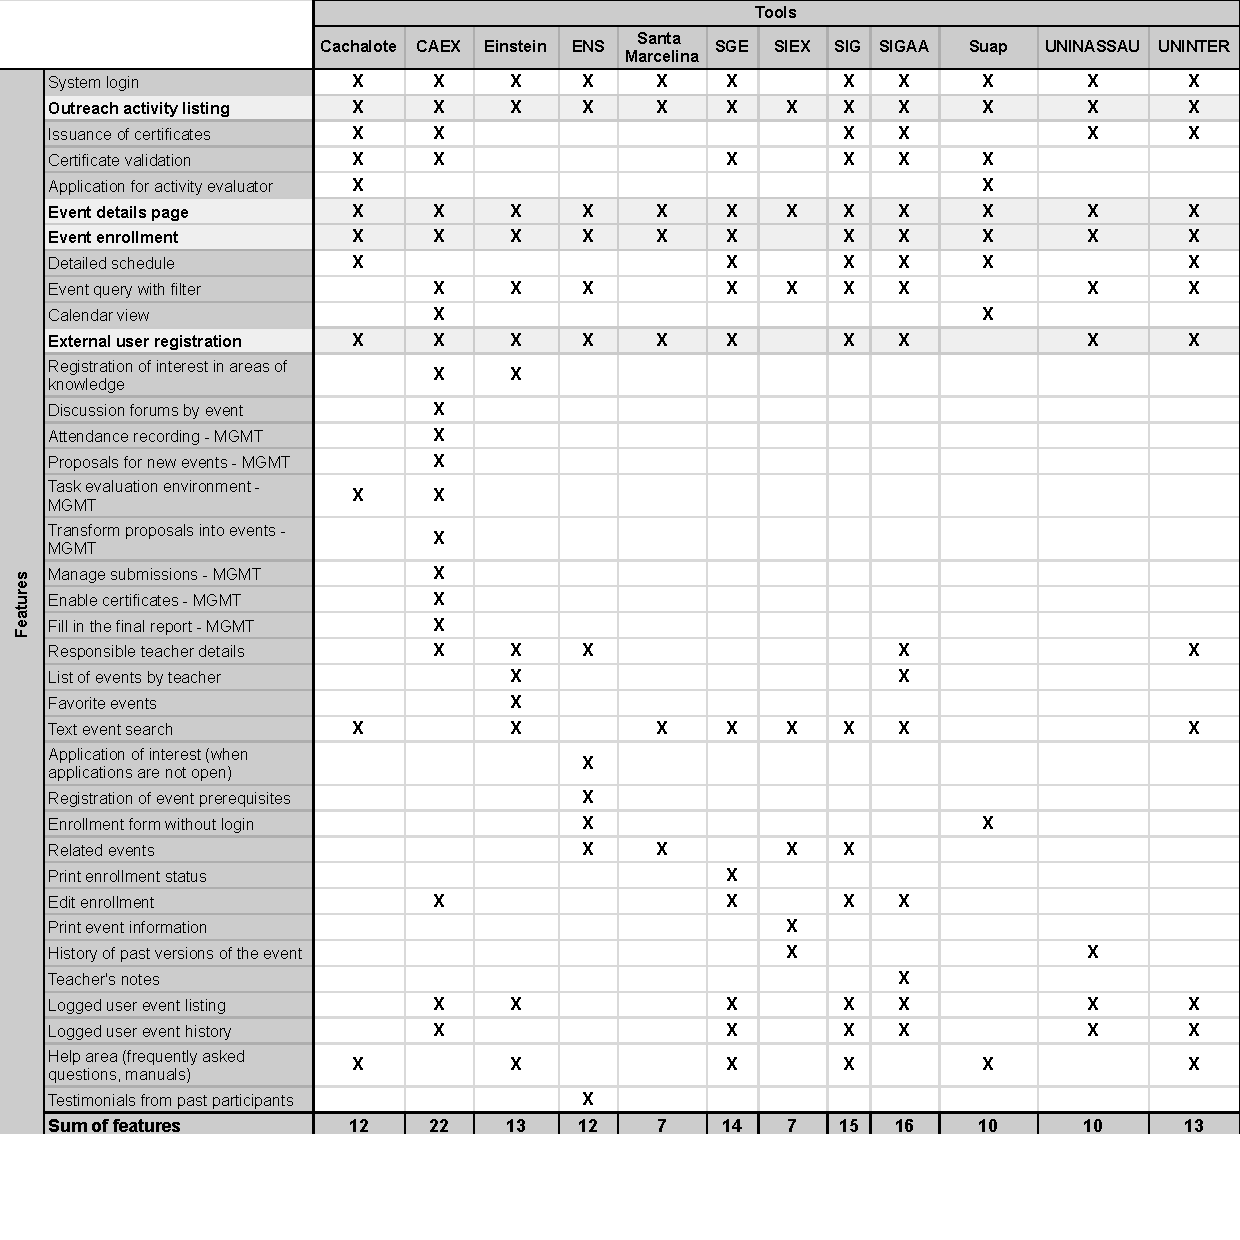
\includegraphics[width=16cm]{img/functionality-matrix.pdf}
  \end{center}
  \fonte{Author.}
\end{figure}

Afterwards, the first four most relevant features in common with all the analyzed tools were highlighted and a new manual extraction was performed. Now with the purpose to find all the features these solutions had. With this data refined and tabulated, it becomes much easier to solve similar problems that will eventually arise when developing the goal product.

\section{Reporting}\label{sec:gl-reporting}

\section{Validity}\label{sec:gl-validity}

\section{Considerations}\label{sec:gl-considerations}